\documentclass[10pt,letterpaper]{article}
\usepackage[margin=1in]{geometry}
\usepackage[T1]{fontenc}
\usepackage{lmodern,microtype,amsmath,amssymb,amsthm,booktabs,array,graphicx}
\microtypesetup{protrusion=false}
\usepackage{xurl}
\usepackage[hidelinks]{hyperref}
\hypersetup{pdftitle={Exact Joint Deformation Costs for Continuous RNA-Ownership Sensitivity},pdfauthor={Arnav Peram}}
\usepackage{enumitem,float,tikz}
\usetikzlibrary{arrows.meta,positioning}
\setlist{nosep,leftmargin=*}
\setlength{\parskip}{3pt}
\setlength{\parindent}{1em}
\renewenvironment{abstract}{\begin{center}\bfseries Abstract\end{center}\begin{quote}\normalsize}{\end{quote}}
\newtheorem{theorem}{Theorem}
\newtheorem{lemma}[theorem]{Lemma}
\newtheorem{proposition}[theorem]{Proposition}
\newcommand{\R}{\mathbb R}
\newcommand{\D}{\mathcal D}
\newcommand{\dist}{\operatorname{dist}}
\newcommand{\ind}{\mathbf 1}
\title{Exact Joint Deformation Costs for Continuous RNA-Ownership Sensitivity}
\author{Arnav Peram}
\date{}
\begin{document}\maketitle
\begin{abstract}
Cell boundaries determine the gene-count profiles measured by imaging-based spatial transcriptomics. Several transcript reassignments can share one boundary displacement, so adding their individual deformation costs can misrepresent the sensitivity of those profiles. We study the minimum continuous deformation realizing each joint assignment in an ordered local cell corridor. For heterogeneous slope limits, thickness bounds, boundary bands, fixed endpoints and nuclear regions, we prove that propagated envelopes admit a simultaneously nearest boundary. Exact integration gives a polynomial-size rational graph preserving this entire assignment-cost function before unary molecular costs are specified. Direct elimination aggregates recurring activation sets without retaining boundary-height choices; an exact critical-mesh construction provides a second representation. Fixed reassignment requests admit a simpler closure algorithm when the source realizes all source-owner constraints. On 42 selected corridors from one Xenium donor, a same-feasibility additive ablation changes the optimum in 1 of 126 baseline and 16 of 126 relaxed-family questions. In the baseline example, a shared displacement of approximately $3.506102\,\mu$m$^2$ transfers five transcripts, switching four genes from detected only in one neighboring cell to detected only in the other. The decision persists over penalties $0.67$--$1.28$ RNA/$\mu$m$^2$. The method supplies exact local gene-count sensitivity witnesses under explicit, uncalibrated geometric assumptions.
\end{abstract}

\section{Introduction: sensitivity of cell-level RNA measurements}
A cell-by-gene count table is a measurement conditioned on a segmentation. A boundary change can move several transcripts together, altering which genes are detected in neighboring cells. Recent benchmarking documents downstream dependence on segmentation choices~\cite{benchmark2026}. A useful sensitivity question is therefore: \emph{how much boundary movement would suffice to change the observed RNA profile, while preserving specified geometric and nuclear constraints?} An attaining boundary makes such a change inspectable; an infeasibility result rules it out within the declared model.

These questions are joint. Two transcripts near the same interface may share the cost of moving it. Conversely, two individually possible transfers may conflict with a slope or cell-thickness constraint. Treating transfers independently loses this dependence. We quantify it by $D^\star(c)$, the smallest integrated boundary displacement realizing the complete assignment vector $c$. The same function supports fixed transfer requests and optimization of additive molecular scores, including fixed-coefficient gene-count contrasts.

The native example illustrates the measurement at stake. Under the original geometric setting, one boundary can transfer five transcripts for approximately $3.506102\,\mu$m$^2$, whereas their separate minimum costs sum to approximately $8.696707\,\mu$m$^2$. Four genes then switch from detected only in the donor cell to detected only in its neighbor. An additive-cost ablation instead transfers one LTBP2 transcript and preserves those four detection calls. The application is a counterfactual audit of the supplied segmentation; its biological use is to identify expression evidence that needs boundary review before interpretation.

\paragraph{Contribution.}
For ordered local boundaries, we construct the entire function $D^\star$, rather than solve continuous geometry afresh for each molecular objective. The central step is \emph{simultaneous attainment}: propagated lower and upper envelopes and the source boundary can be clamped coordinatewise while remaining jointly feasible. The resulting boundary attains every pointwise nearest displacement. We then integrate its cost exactly. Two finite reductions follow: a derived critical mesh retaining heights, and a direct representation retaining assignment bits and integrated cost helpers. Counting distinct activation prefixes bounds the direct helper graph by $O(N^2m^5)$; source-curve detail still enters integration work and coefficient size. The comparison between these reductions measures representation overhead. The additive ablation separately tests the information lost by removing shared deformation.

\paragraph{Relation to graph-cut methods.}
Ordered-label and convex-prior optimization~\cite{ishikawa,hochbaum}, interacting-surface cuts~\cite{li,shah}, and higher-order auxiliary-variable reductions~\cite{kz,kohli} supply established machinery. After integration, our excursion energy is a weighted coverage function, implemented with standard OR helpers. General submodularity alone would not guarantee such a reduction~\cite{zivny}; here the explicit coverage decomposition supplies it. Lattice closure~\cite{felsner}, Lipschitz envelopes~\cite{petrakis,agarwal} and functional lifting~\cite{pock} are also foundations. The result to assess is the constructive elimination of this continuous, coupled assignment geometry and its ownerwise cost identity, together with the aggregated size bound.

\paragraph{Relation to spatial-transcriptomics methods.}
Baysor and Proseg estimate assignments~\cite{baysor,proseg}; BIDCell uses biologically informed segmentation losses~\cite{bidcell}; Segger formulates transcript--cell association as link prediction~\cite{segger}. ResolVI models misassignment and other nuisance effects probabilistically~\cite{resolvi}, while ovrlpy diagnoses vertical signal overlap~\cite{ovrlpy}. Our output is a deformation witness or exclusion under a chosen local geometry. These different output objects motivate complementary use after segmentation. The present evaluation audits source Xenium masks and isolates shared cost; evaluating corrected ownership against alternative segmentation tools requires an additional accuracy study.

\section{A local geometric model}\label{sec:model}
\noindent A \emph{corridor} is a small patch in which cells keep a fixed left-to-right order. A boundary height is its horizontal position as the vertical coordinate varies. Assigning a transcript to a cell imposes lower or upper boundary restrictions, called \emph{obligations}; propagation spreads these restrictions through slope and thickness constraints.\par
Let $m$ functions $f_a:I\to\R$, $I=[t_-,t_+]$, partition a rectangle into $m+1$ ordered cells. Boundary $a$ is $s_a$-Lipschitz, $s_a>0$, lies in a constant band $[\underline b_a,\overline b_a]$, and has fixed endpoint values. Adjacent boundaries satisfy
\begin{equation}
 0<d_a^{\min}\le f_{a+1}(t)-f_a(t)\le d_a^{\max}.\label{eq:gap}
\end{equation}
The upper bound may be absent. A rational piecewise-linear source $f^0$ obeys these geometric constraints. Fixed exterior rails beyond the bands make all strips connected and nonempty. This coordinate model excludes arbitrary tessellations, branching boundaries, triple junctions, and holes.

Each site $i$ is a rectangle $[x_i^-,x_i^+]\times I_i$, including zero-size point sites, in group $g(i)$. A group receives one owner $c_g\in\{0,\ldots,m\}$. Its nested threshold bits are
\begin{equation}
 b_{ga}=\ind[c_g\le a],\qquad b_{ga}\le b_{g,a+1}.\label{eq:bits}
\end{equation}
With horizontal clearance $\rho>0$, ownership of the entire location rectangle (\emph{universal-region} ownership) imposes
\begin{align}
 b_{g(i),a}=1&\ \Longrightarrow\ f_a(t)\ge\ell_i=x_i^++\rho &&(t\in I_i),\nonumber\\
 b_{g(i),a}=0&\ \Longrightarrow\ f_a(t)\le u_i=x_i^--\rho &&(t\in I_i).\label{eq:obligations}
\end{align}
One boundary and owner must work for every position in the rectangle. Nominal mode uses its center. A fixed nuclear rectangle always uses~\eqref{eq:obligations}, has a pinned cell owner, and has no RNA cost. Compatible structural rectangles with the same owner and transverse interval may be merged by their exact union. An incompatible nuclear region makes the model infeasible.

For rational unary costs $C_g(c)$ and $\lambda\ge0$, optimize
\begin{equation}
 E^*=\min_{f,c}\left\{\lambda\D(f)+\sum_g C_g(c_g)\right\},\qquad
 \D(f)=\sum_a\int_I |f_a-f_a^0|\,dt.\label{eq:objective}
\end{equation}
RNA groups may contain multiple charged molecules. Fixed-coefficient regional gene counts are unary objectives; changing-denominator pairwise ratios, top-$k$ membership loss, and general hard-budget optima are not automatically covered. Units must be supplied consistently. $\D$ is \emph{summed interface displacement}: for ordered cell-index functions $c_f$,
\begin{equation}
 \D=\iint|c_f-c_{f^0}|\,dx\,dt,\qquad A_{\rm changed}\le\D\le m A_{\rm changed}.\label{eq:area}
\end{equation}
With several interfaces, a tissue location can be charged more than once. Geometric settings and location regions specify a sensitivity family.

\section{Exact finite elimination of continuous geometry}\label{sec:theory}
\subsection{How a boundary restriction constrains its neighbors}
Create a boundary-index graph with $a\to a+1$ of weight $d_a^{\min}$ and, when finite, $a+1\to a$ of weight $-d_a^{\max}$. Let $\Delta_{ab}$ be its maximum path weight, with $\Delta_{aa}=0$ and $-\infty$ for no path. Source feasibility excludes positive cycles. Max-plus Floyd--Warshall computes $\Delta$ in $O(m^3)$ arithmetic operations. Define
\begin{equation}
 K_{ab}(r)=\max_c\{\Delta_{ac}+\Delta_{cb}-s_c r\},\qquad r\ge0,\label{eq:kernel}
\end{equation}
using only existing paths.

\begin{lemma}[Propagation closure]\label{lem:kernel}
Every admissible family satisfies $f_b(v)\ge f_a(u)+K_{ab}(|u-v|)$. This is the strongest inequality obtained by finite composition of the given longitudinal Lipschitz and same-coordinate separation constraints.
\end{lemma}
\begin{proof}
For each $c$, transfer from $a$ to $c$ at $u$, travel to $v$ on $c$, then transfer to $b$. Conversely, in any composite path choose a surface $c$ of minimum slope among the longitudinal steps. Its vertical steps before and after that visit total at most $\Delta_{ac}+\Delta_{cb}$. Its absolute longitudinal travel is at least $|u-v|$, at rates at least $s_c$. Its implied bound cannot exceed that term of~\eqref{eq:kernel}. Zero longitudinal travel is covered at $r=0$.
\end{proof}
Thus $K_{ab}(0)=\Delta_{ab}$, kernels are nonincreasing, and
\begin{equation}
 K_{ab}(r_1+r_2)\ge K_{ac}(r_1)+K_{cb}(r_2).\label{eq:composition}
\end{equation}
A destination-$b$ term with rate $s_c>s_b$ is dominated by the direct $b$ term, since $\Delta_{ac}+\Delta_{cb}\le\Delta_{ab}$. The corresponding source statement holds as well. These observations ensure the required propagated slopes.



\subsection{Finite constraints for realizable assignments}
For a lower obligation $(a,I_i,\ell_i)$, forbid its activating bit value $1$ if, for any destination $b$ and kernel term $(d,s)$ of $K_{ab}$,
\begin{equation}
 \ell_i+d>\overline b_b\quad\text{or}\quad
 \ell_i+d>f_b^0(e)+s\dist(e,I_i)\quad\text{for }e\in\{t_-,t_+\}.\label{eq:unarylower}
\end{equation}
For an upper obligation $(a,I_i,u_i)$, forbid activating value $0$ if a term $(d,s)$ of $K_{ba}$ satisfies
\begin{equation}
 u_i-d<\underline b_b\quad\text{or}\quad
 f_b^0(e)>u_i-d+s\dist(e,I_i).\label{eq:unaryupper}
\end{equation}
For every ordered lower/upper pair add
\begin{equation}
 b_{g(i),a}\Longrightarrow b_{g(j),b}
 \quad\text{if}\quad \ell_i+K_{ab}(\dist(I_i,I_j))>u_j.\label{eq:implication}
\end{equation}
Same-bit implications are tautologies. Add~\eqref{eq:bits} and pins $b_{ga}=\ind[c_g^{\rm fixed}\le a]$ for all structural groups. Equations~\eqref{eq:unarylower}--\eqref{eq:implication} apply to RNA and pinned structures identically. Contradictory unary fixes or implications mean model infeasibility.

\begin{theorem}[Exact ownership feasibility]\label{thm:feas}
The finite restrictions above characterize exactly the universal-region owner vectors realizable in the declared continuous family.
\end{theorem}
\begin{proof}
Necessity follows from Lemma~\ref{lem:kernel}, using the smallest interval distance for a nonincreasing kernel. For sufficiency, propagate selected lower and upper obligations into envelopes $L_b,U_b$. Their molecular contributions are
\[
 \ell_i+K_{ab}(\dist(t,I_i)),\qquad
 u_j-K_{ba}(\dist(t,I_j)),
\]
respectively. Include fixed endpoints as both lower and upper point data; include bands as interval data across all of $I$. Equation~\eqref{eq:composition}, the triangle inequality, and~\eqref{eq:implication} put every lower contribution below every upper contribution; the unary tests handle their comparisons to fixed data. Hence $L_b\le U_b$. For every directed separation edge $a\to b$ of weight $d$, closure gives $K_{ob}\ge K_{oa}+d$, hence $L_b\ge L_a+d$. Similarly $K_{ao}\ge d+K_{bo}$ implies $U_a\le U_b-d$. Applying this to both directed edges enforces both finite gap bounds, not just the minimum. Dominated rates preserve each surface's Lipschitz bound. Fixed data enforce bands and endpoint equality. Thus the envelopes are feasible realizations. Nesting specifies exactly one cell per group.
\end{proof}
For example, when two boundaries have fixed separation one, slopes two and $1/4$, and fixed source heights zero and one, the left boundary can reach at most $1/8$ at distance $1/2$ from the endpoint. Its own slope alone would give the incorrect limit one. This demonstrates why a neighboring regularity constraint cannot be ignored.

\subsection{A nearest boundary and its integrated cost}
For an owner vector $c$, define
\[
 D^\star(c)=\min_{f\in\mathcal F(c)}\D(f),
\]
with $+\infty$ for an empty realization family.
\begin{theorem}[Ownerwise integrated-cost representation]\label{thm:cut}
For rational input, a polynomial-size directed graph $G_D$ with molecular threshold vertices $b(c)$, auxiliary vertices $y$, and hard arcs satisfies:
\begin{enumerate}
\item A hard-feasible cut with molecular labels $b(c)$ exists exactly when $\mathcal F(c)\ne\varnothing$.
\item For \emph{every} such owner vector, before choosing molecular costs,
\begin{equation}
 \min_y\operatorname{Cut}_{G_D}(b(c),y)+\kappa=D^\star(c).\label{eq:ownerwise}
\end{equation}
\end{enumerate}
Here $\kappa$ is an explicitly recorded rational constant, initially zero; capacities are rational. After common-denominator scaling, divide the integer cut value by that scale. Consequently, for arbitrary rational unary costs and rational $\lambda\ge0$, one finite cut either detects model infeasibility or returns optimal owners and an attaining rational piecewise-linear boundary for~\eqref{eq:objective}.
\end{theorem}
\begin{proof}
For any feasible owner vector, set
\begin{equation}
 f_b^*(t)=\min\{U_b(t),\max\{L_b(t),f_b^0(t)\}\}.\label{eq:clamp}
\end{equation}
Families satisfying lower difference inequalities are closed under componentwise min and max: from $f_b\ge f_a+d$ and $g_b\ge g_a+d$ both operations preserve the inequality. Min/max also preserve scalar Lipschitz bounds, bands, and endpoints. Hence~\eqref{eq:clamp} is feasible. Every realizing boundary lies in $[L_b,U_b]$ pointwise; the clamp is its nearest point to $f_b^0$. It therefore minimizes each absolute displacement and their integrated sum.

A propagated restriction has a tent-shaped profile, called a cone. The upward displacement is a maximum of nonnegative functions
\[
 [\ell_i+d-s\dist(t,I_i)-f_b^0(t)]_+
\]
activated by bits; downward functions are activated by complementary bits. Fixed geometric data already satisfied by $f^0$ cannot push it outward. Selected structural and RNA obligations are retained even when they are not nominal flips: the source need not satisfy every uncertain RNA rectangle. Upward and downward displacement cannot both be positive for feasible owners.

Split $I$ at plateau endpoints, source knots, zeros, and positive pair intersections. On a slab, positive affine heights have fixed order $h_1\ge\cdots\ge h_k>0$, with $h_{k+1}=0$. For activated groups, their maximum is exactly
\begin{equation}
 \sum_{j=1}^k(h_j-h_{j+1})\ind[\text{at least one of the top-$j$ activations holds}].\label{eq:layers}
\end{equation}
Integrate each affine difference rationally. Positive OR layers use a helper $z$, hard arcs $b\Rightarrow z$, and a helper-to-sink capacity. Complement OR layers use $z\Rightarrow b$ and a source-to-helper capacity. Repeated activations are not independent variables. Nested sets share predecessor helpers, giving constant arcs per distinct layer. These are standard higher-order reduction gadgets~\cite{kz,kohli}; their weights here are exact geometric integrals.

Finally,
\begin{equation}
 C_g(c_g)=C_g(m)+\sum_{a=0}^{m-1}[C_g(a)-C_g(a+1)]b_{ga}.\label{eq:unary}
\end{equation}
Shift negative unaries by a recorded constant and include all feasibility/pin arcs. Before unaries are added, minimization over the OR helpers yields exactly the integrated clamp displacement for each fixed $b(c)$, proving~\eqref{eq:ownerwise}. Adding~\eqref{eq:unary} and $\lambda$ therefore preserves the minimum of~\eqref{eq:objective}. Recover owners and~\eqref{eq:clamp}. Scaling rational capacities by a common denominator permits integer flow/cut proofs; hard capacity one greater than the sum of finite capacities ensures a hard-arc cut occurs only when the pinned model is infeasible.
\end{proof}


\paragraph{Aggregated graph size and encoding.}
Let $N$ count all merged obligation rectangles, including pinned nuclear structures; $G$ counts groups. On boundary $b$ there are $M_b=O(Nm^2)$ propagated cone terms across both polarities and $J_b$ source knots. A direct arrangement can have $Q_b=O(M_b^2+M_bJ_b+J_b+1)$ slabs, but charging every prefix on every slab overcounts the \emph{aggregated graph}.

For one polarity, write the untruncated cone terms as $g_i(t)=\alpha_i-s_i\dist(t,I_i)$. Subtracting or adding a common source does not change their relative order. Each pair of constant-piece affine cones changes order only constantly many times. Resolve simultaneous events into adjacent swaps; each swap changes only one full prefix set. Starting with $M_b$ prefixes therefore yields $O(M_b^2+M_b)$ distinct sets. Positivity selects some of these prefixes, and repeated activation labels cannot increase their count. Retaining zero-weight predecessors as necessary gives a constant-arc helper construction. Thus
\begin{align}
 |V_{\rm cut}|&=O\!\left(Gm+\sum_b(M_b^2+M_b)\right),\nonumber\\
 |E_{\rm cut}|&=O\!\left(Gm+N^2m^2+\sum_b(M_b^2+M_b)\right).\label{eq:size}
\end{align}
The auxiliary-size contribution is $O(N^2m^5)$. This is a representation bound, not a faster implementation claim: the current compiler still scans slab layers before merging. Source knots affect integration work, rational coefficient length, and reconstruction. The supplement treats ties, repeated labels and helper predecessors explicitly.

All rationals are binary encoded. Closure weights use simple paths; intersections, affine integration and sums have polynomial bit complexity. A common capacity denominator has bit length at most the sum of its constituent denominator lengths. Group-set bookkeeping and construction work remain polynomial and can be large. No asymptotic dominance over every compressed height representation follows.

\paragraph{An exact critical-mesh alternative.}
For each boundary, collect every propagated lower/upper obligation piece, fixed geometric piece, and source piece, before choosing owners. A common mesh contains their breakpoints and all same-boundary crossings. On every mesh interval, the canonical clamp for \emph{any} feasible ownership vector selects one affine piece and its displacement has constant sign. Its trapezoidal cost is exact. Conversely, interpolating any feasible nodal vector preserves the linear constraints, and its trapezoidal absolute-displacement cost upper-bounds its integral. Because the canonical minimizer is included, the nodal minimum equals $D^\star(c)$ for every $c$.

Restrict each nodal height to the candidate-function values there. The same canonical minimizer remains available. Ordered height bits encode each choice; slope, thickness and ownership inequalities become implications, and trapezoidal weights are unary nodal costs. This is a second exact surface-cut reduction. The supplement gives the full construction, safe pin-envelope pruning, and a polynomial size bound. It uses absolute displacement; exact trapezoids are not asserted for higher loss powers. The direct graph instead integrates activation layers across intervals and can merge recurring activation sets. Neither construction is claimed to dominate all possible compressed surface representations.

\section{Fixed transfer requests and jointly chosen assignments}\label{sec:queries}
\subsection{Minimum movement for specified transfers}
A \emph{pinned} query prescribes selected transcript owners and minimizes movement over the remaining choices. An \emph{optional} query chooses owners by balancing movement against molecular costs.

Assume now that the source $f^0$ realizes its complete source bit vector $b^0$, including all structural and molecular obligations, at zero deformation. Geometric source feasibility alone is insufficient: this stronger condition can fail for universal RNA regions.

\begin{proposition}[Source-clipped pin optimum]\label{prop:pin}
Assume $f^0$ satisfies \emph{every source-owner obligation}, including molecular regions and structural pins, at zero deformation. Add owner pins to the implication system in Theorem~\ref{thm:feas}. Propagate forced ones forward and forced zeros backward, obtaining sets $T$ and $F$. If they intersect, the pinned problem is infeasible. Otherwise the assignment
\[
 \widehat b_v=1\ (v\in T),\qquad \widehat b_v=0\ (v\in F),\qquad
 \widehat b_v=b_v^0\ (v\notin T\cup F)
\]
minimizes $D^\star$ over all pinned completions. Its cost and attaining curves follow from fixed-owner envelope reconstruction; no integrated-cost layers or weighted minimum cut are needed.
\end{proposition}
\begin{proof}
The least pinned assignment has ones exactly in $T$ and the greatest has zeros exactly in $F$. The implication family is closed under componentwise minimum and maximum, so clipping the feasible $b^0$ between these extremes produces a feasible pinned vector. Any obligation unchanged from $b^0$ contributes zero positive source-relative excursion because $f^0$ satisfies it and all propagated geometry. Every nonzero excursion activated by $\widehat b$ comes from a forced change and is activated by every pinned completion. Additional optional changes cannot remove these functions from either polarity's maximum. Consequently the envelope displacement of $\widehat b$ is pointwise no greater than that of any completion. Integrating proves the minimum.
\end{proof}
Preparation constructs the ownership implication system and checks source admissibility once. A query traverses implications and reconstructs envelopes. A contradiction path proves infeasibility. This is a corollary of the representation's order structure, not a new general closure algorithm. The general compiler supports arbitrary unary optimization, but is not needed for these pinned queries. The implementation explicitly refuses source-clipping when its stronger premise fails.

\subsection{The cost of moving transcripts together}
Assume again that $f^0$ realizes \emph{all source-owner obligations and structural pins at zero deformation}. For a fixed corridor $\mathcal C$, define $d_{g\to j\mid\mathcal C}$ as the minimum deformation under the pin $c_g=j$, with every other RNA free. Set the source-owner cost to zero. For any jointly feasible $c$,
\begin{equation}
 D^\star(c)\le A(c):=\sum_g d_{g\to c_g\mid\mathcal C}.\label{eq:upperadd}
\end{equation}
Each single-pin completion contains the obligations forced by that pin. The least source-relative completion of all pins contains their union. Its positive and negative excursion maxima are bounded by the sum of the singleton maxima. A complete vector pins every owner, so integrating proves~\eqref{eq:upperadd}. This upper bound can be strict; it is not an equality model.

Take one boundary on $[0,3]$, zero source and endpoints, slope bound one, band $[-1/2,1/2]$, and two right-owned sites $(1/5,1)$ and $(1/5,5/4)$ with clearance $1/20$. All four owner patterns are feasible. Each singleton costs $1/16$, while both cost $7/64$. At reward $3/50$ per change the singleton objective is positive, but the joint objective is $-17/1600$. The additive surrogate preserves both owners; the joint objective changes both. Figure~\ref{fig:reduction} shows the two exact encodings. Moving the second ordinate to $2$ preserves singleton costs and feasibility but removes the shared saving, establishing that these marginals do not determine the joint decision.

\begin{figure}[t]\centering
{\normalsize $g_1(t)=[\tfrac14-|t-1|]_+$,\quad $g_2(t)=[\tfrac14-|t-\tfrac54|]_+$,\quad
$D^\star(x)=\int\max(x_1g_1,x_2g_2)\,dt$}\par\medskip
\begin{minipage}[c]{.50\linewidth}\centering
\textbf{Exact height expansion}\\[4pt]
\begin{tabular}{cc}\toprule
Mesh coordinate & Canonical candidates\\\midrule
$3/4$ & $0$\\
$1$ & $0,1/4$\\
$9/8$ & $0,1/8$\\
$5/4$ & $0,1/4$\\
$3/2$ & $0$\\\bottomrule
\end{tabular}
\end{minipage}\hfill
\begin{minipage}[c]{.47\linewidth}\centering
\textbf{Integrated owner layers}\\[3pt]
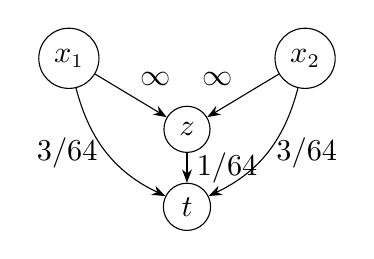
\begin{tikzpicture}[x=1cm,y=.82cm,>=Stealth,every node/.style={font=\fontsize{10.5}{12}\selectfont}]
\node[draw,circle] (a) at (0,1.3) {$x_1$};
\node[draw,circle] (b) at (3,1.3) {$x_2$};
\node[draw,circle] (z) at (1.5,.2) {$z$};
\node[draw,circle] (t) at (1.5,-1) {$t$};
\draw[->] (a)--node[above right] {$\infty$}(z);
\draw[->] (b)--node[above left] {$\infty$}(z);
\draw[->] (z)--node[right] {$1/64$}(t);
\draw[->] (a) to[bend right=25] node[left] {$3/64$}(t);
\draw[->] (b) to[bend left=25] node[right] {$3/64$}(t);
\end{tikzpicture}
\end{minipage}
\caption{A constructed two-site reduction. Height choices retain a canonical boundary; direct layers integrate them into $D^\star(x)=3(x_1+x_2)/64+\operatorname{OR}(x_1,x_2)/64$. Source-side cut labels equal one; the sink is $t$. Both recover costs $0,1/16,1/16,7/64$. The middle height encodes shared excursion, which becomes the helper $z$.}\label{fig:reduction}
\end{figure}

\subsection{An ablation of shared deformation}
We compare the joint-model objective $E(c)=\lambda D^\star(c)-R(c)$ with
$E_A(c)=\lambda A(c)-R(c)$, where $R$ counts all included reassigned RNAs. The surrogate retains \emph{exactly the same} implications, structural pins, and owner set. Infinite singleton alternatives are excluded by those same constraints. To avoid counting arbitrary ties as failures, among \emph{all} $E_A$ minimizers we choose one minimizing the joint-model $E$.

This secondary optimization is exact. Let $L$ integer-scale all rational surrogate unary costs, and choose integer $M>\lambda B+W$, where $B=|I|\sum_a(\overline b_a-\underline b_a)$ bounds deformation and $W$ is total RNA weight. Minimize $ML E_A+E$ using the joint-cost compiler. Distinct primary values differ by at least $1/L$, whereas the entire joint-model objective range is at most $\lambda B+W$. The larger primary coefficient enforces exact lexicographic order. Thus positive reported regret holds even after giving the surrogate the most favorable joint-model tie choice. This control is an evaluation device, not a deployable shortcut replacing the joint-model objective.

\section{Native gene-count sensitivity}\label{sec:native}
\subsection{Data, selection and geometric settings}
We use two existing development crops from one public Xenium human lung-cancer donor~\cite{data,xenium}. The 42 selected corridors contain 464 repeated RNA records, 387 distinct transcripts and 51 source cells: 34 two-cell and eight three-cell corridors. The source crops contain 7,370 Q20 gene transcripts. The amended extraction uses fixed height/orientation screens, a deterministic hash order and per-setting caps; selection is documented in the supplement. The retained ordered patches cover approximately 5.25\% of the distinct crop transcripts. Their results concern local compatible interfaces, with junctions and branching topology outside the model.

Baseline bands extend the source range by $0.5\,\mu$m; slopes are at least one and cover the source slopes. Gap bounds are one-half the minimum and twice the maximum source separation; clearance is $0.001\,\mu$m. The largest declared family doubles slopes and band padding and extends both endpoints by half the original corridor length, keeping observations and nuclear regions fixed. These settings are declared perturbations rather than anatomical estimates. All analyses retain the same 42 corridors, both settings and penalties $\lambda\in\{1/4,1,4\}$ RNA/$\mu$m$^2$.

\subsection{Shared cost changes a native reassignment decision}
The objective $\lambda D^\star-R$ rewards the number $R$ of source-owner changes while charging their joint deformation. It asks how much coordinated instability a supplied geometry permits. The additive ablation replaces $D^\star$ by the sum of exact individual transfer costs, retaining the identical feasible assignments. Among all additive minimizers it receives the best joint-model objective. Thus strict regret reflects the discarded shared cost.

\begin{table}[t]\centering
\begin{tabular}{lrrrr}\toprule
Setting & Questions & Strict regret & Affected corridors & Joint cost below sum\\\midrule
Baseline &126&1&1&18\\
Largest family &126&16&12&48\\\bottomrule
\end{tabular}
\caption{Complete ablation census. ``Below sum'' refers to the joint optimizer's assignments. The 235 zero-regret cases remain included; sharing need not change the selected optimum.}\label{tab:joint}
\end{table}

The ablation is strictly worse in 1/126 baseline and 16/126 enlarged-family questions (Table~\ref{tab:joint}); all 17 change the reassignment count. These are dependent questions on development data. The ablation isolates a modeling choice; it is not an existing segmentation algorithm. The largest joint-objective regret is approximately 1.43357.

At the original $\lambda=1$ in baseline corridor \texttt{4037abe9fea38e}, the joint solution transfers one PECAM1, TMEM100, MYC, C7 and PMP22 transcript from cell 153133 to 153124. Their separate costs sum to approximately $8.696707\,\mu$m$^2$, while one shared movement realizes all five for approximately $3.506102\,\mu$m$^2$. The additive minimizer instead transfers one LTBP2 transcript in the opposite direction for approximately $0.779423\,\mu$m$^2$. Their joint-model objectives are approximately $-1.493898$ and $-0.220577$, a regret of approximately $1.273321$.

\begin{figure}[t]\centering
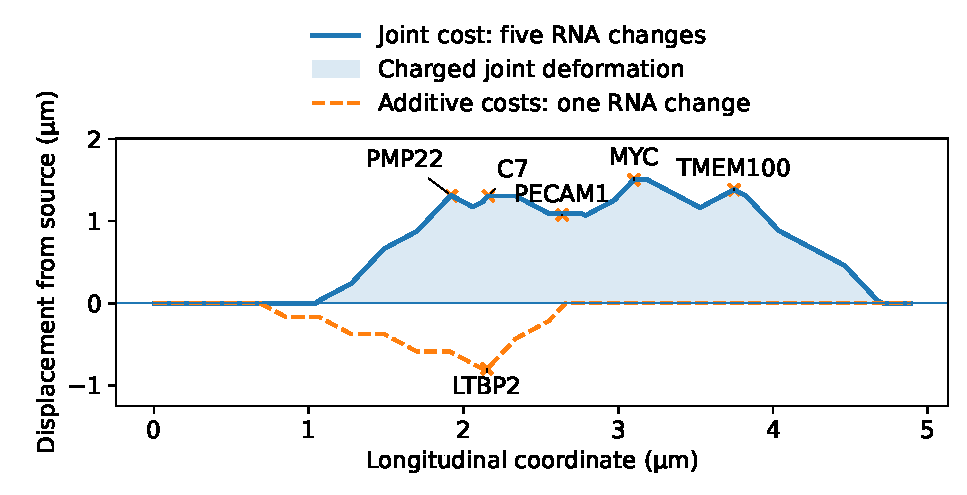
\includegraphics[width=.96\linewidth]{figures/native_joint_displacement.pdf}
\caption{Source-relative boundary displacement in the baseline example. The shaded movement transfers five transcripts together. The dashed additive-optimal boundary transfers LTBP2 alone. Both satisfy the same nuclear and geometric constraints. These are attaining sensitivity alternatives to the supplied segmentation.}\label{fig:native}
\end{figure}

A separate rational implementation enumerates all 64 candidate vectors, recovers 26 feasible ones and agrees on every cost. Both selected assignments are uniquely optimal for their respective objectives throughout $0.67\le\lambda\le1.28$. Every competing affine objective has positive gaps at both endpoints. The additive selection's joint-objective regret is approximately $4-2.726679\lambda$, exceeding $0.50985$ throughout this interval. This is fixed-geometry penalty stability. The example was selected after the full census for illustration.

\subsection{Consequences for the observed cell-by-gene table}
We re-read the retained crop Parquet files with PyArrow, verify every transcript's source-mask label and all 464 corridor records, and count all retained genes by source cell. For each of the 252 original questions, we update only its corridor transcripts and hold other assignments fixed. We then compare counts and the elementary detection indicator $\mathbf1[\text{count}>0]$. This post-hoc readout analysis retains every question and gene, with no marker panel or geometric retuning.

\begin{table}[H]\centering
\begin{tabular}{lrrr}\toprule
Gene & Source counts & Joint alternative & Additive alternative\\
 & (153124,153133) & (153124,153133) & (153124,153133)\\\midrule
PECAM1 &$(0,1)$&$(1,0)$&$(0,1)$\\
TMEM100 &$(0,1)$&$(1,0)$&$(0,1)$\\
MYC &$(0,1)$&$(1,0)$&$(0,1)$\\
C7 &$(0,1)$&$(1,0)$&$(0,1)$\\
PMP22 &$(1,1)$&$(2,0)$&$(1,1)$\\
LTBP2 &$(5,1)$&$(5,1)$&$(4,2)$\\\bottomrule
\end{tabular}
\caption{Observed Q20 gene counts in the baseline example, with all other assignments held fixed. Both cell masks lie wholly inside the source crop. The joint alternative removes all observed copies of five genes from cell 153133 and introduces four previously undetected genes into cell 153124. Counts describe an admissible alternative, not an inferred correction.}\label{tab:readout}
\end{table}

Table~\ref{tab:readout} connects the shared movement to a cell-level readout. The source cells contain 20 and 30 retained transcripts; the joint alternative gives 25 and 25. The additive alternative gives 19 and 31 and preserves the displayed detections. The joint witness therefore shows that these four cell-specific gene detections are not invariant at the showcased exact deformation (approximately $3.506102\,\mu$m$^2$). It supplies an attainable counterexample, without claiming a general hard-budget optimizer or a biological cell-type transition.

Across the full census, returned joint optima change at least one detection indicator in 47/126 baseline and 88/126 enlarged-family questions; restricting the readout to masks wholly within a crop gives 45 and 85. Joint and tie-favorable additive answers differ in detection indicators in the one baseline regret case and 13 of the 16 enlarged-family regret cases. These numbers characterize returned alternatives; ties outside the unique showcase may admit other count tables. The supplement provides all cases and distinguishes detection changes from expression accuracy.

\section{Computation and verification}\label{sec:resources}
Both implementations compile each of the same 84 corridor/setting models once and solve its three optional objectives. The height construction receives the same feasibility closure and envelope pruning. Both receive identical contraction of strongly connected components (SCCs) of hard implications, whose vertices must share a cut label. This preserves every feasible cut cost. Compilation, flow, lifting, exact reconstruction and checking are timed; parsing and imports are excluded.

\begin{table}[t]\centering
\begin{tabular}{lrrr}\toprule
Exact workflow & Sum of vertices & Sum of arcs & Median total (s)\\\midrule
Direct owner layers &1,806&13,212&4.266\\
Critical-mesh heights &37,052&149,120&25.928\\
Direct + hard SCCs &1,431&7,855&4.530\\
Height + hard SCCs &6,473&27,010&19.540\\\bottomrule
\end{tabular}
\caption{Three fresh processes per condition on 84 separate local graphs and 252 objectives. Every objective agrees exactly. These are two implementations of the same energy, with a shared integer-flow backend.}\label{tab:optional_runtime}
\end{table}

After contraction, the height/direct median-total ratio is 4.31; the query-and-check ratio is 1.58. Compilation accounts for most of the difference. All 48 models retaining optional owners favor direct, with median per-model ratio 3.88. All 36 fixed models favor height, with ratio 0.445, because it caches their boundary whereas direct reconstructs each time. Both groups enter Table~\ref{tab:optional_runtime}. The native graphs are small (at most 76 uncontracted direct vertices); this experiment measures representation overhead, not atlas-scale performance. The supplement retains a constructed five-cell, 384-group compilation timeout as a scalability limitation.

For all 1,132 fixed transfer queries, source clipping reproduces the graph answers in 4.611 seconds, versus 5.618 for graph reuse; detailed checks and timings appear in the supplement.

\paragraph{Verification.}
Integer flow certificates establish finite-graph optimality. Direct geometric checks establish continuous feasibility and attained area. Separate ownerwise enumeration and the height construction test the reduction. The new readout census freshly solves 756 joint, additive-primary and favorable-tie objectives and passes 1,008 archived objective/regret checks. Gene-count updates also conserve each gene's total across the affected cells. 

\section{Use, limitations and availability}
The method supplies a realizable changed RNA profile and its least boundary cost, or excludes a transfer within the model. The ownerwise representation preserves shared deformation before unary molecular costs are chosen.

The main limits are structural and empirical. Ordered corridors exclude junctions and general tessellations; the selected one-donor data and uncalibrated parameters do not establish biological prevalence. The 1/126 baseline result supports a mechanism rather than routine superiority of joint over additive costs. Thresholds depend on the corridor, its retained observations and its neighboring cells: among 54 repeated transcript/source/destination combinations, the largest setting has three feasibility disagreements and four finite-cost differences. Next, extraction and calibration should be fixed before testing sensitivity against independent segmentation or imaging evidence on held-out tissue.

\paragraph{Availability and AI assistance.}
Documented source, inputs and readout scripts are public at \url{https://github.com/arnavperam/geocert}, revision \href{https://github.com/arnavperam/geocert/tree/fdffadfedc0e21202d554c8425add3349199a766}{\texttt{fdffadfedc0e}}; its exact core is unchanged from release \texttt{1.0.0}. An artifact map links all current and historical studies. Generative AI assisted implementation, computational checks, methodological discussion and manuscript revision; responsibility for the submitted claims remains with the author.

\clearpage
\begin{thebibliography}{99}
\bibitem{baysor} V. Petukhov et al. Cell segmentation in imaging-based spatial transcriptomics. \emph{Nature Biotechnology} 40:345--354, 2022. doi:10.1038/s41587-021-01044-w.
\bibitem{proseg} D. C. Jones, A. E. Elz, A. Hadadianpour, H. Ryu, D. R. Glass, and E. W. Newell. Cell simulation as cell segmentation. \emph{Nature Methods} 22:1331--1342, 2025. doi:10.1038/s41592-025-02697-0.
\bibitem{li} K. Li, X. Wu, D. Z. Chen and M. Sonka. Optimal surface segmentation in volumetric images---a graph-theoretic approach. \emph{IEEE TPAMI} 28(1):119--134, 2006. doi:10.1109/TPAMI.2006.19.
\bibitem{shah} A. Shah, M. D. Abramoff and X. Wu. Optimal surface segmentation with convex priors in irregularly sampled space. \emph{Medical Image Analysis} 54:63--75, 2019. doi:10.1016/j.media.2019.02.004.
\bibitem{petrakis} I. Petrakis. McShane--Whitney extensions in constructive analysis. \emph{Logical Methods in Computer Science} 16(1):18, 2020. doi:10.23638/LMCS-16(1:18)2020.
\bibitem{kz} V. Kolmogorov and R. Zabih. What energy functions can be minimized via graph cuts? \emph{IEEE TPAMI} 26(2):147--159, 2004. doi:10.1109/TPAMI.2004.1262177.
\bibitem{data} 10x Genomics. Preview Data: FFPE Human Lung Cancer with Xenium Multimodal Cell Segmentation. 5 February 2024. One donor; CC BY 4.0. \url{https://www.10xgenomics.com/datasets/preview-data-ffpe-human-lung-cancer-with-xenium-multimodal-cell-segmentation-1-standard}.
\bibitem{xenium} 10x Genomics. Understanding Xenium Outputs: cell and nucleus segmentation files. Documentation accessed 26 October 2026. \url{https://www.10xgenomics.com/support/software/xenium-onboard-analysis/3.2/analysis/xoa-output-understanding-outputs}.
\bibitem{agarwal} P. K. Agarwal, J. M. Phillips and B. Sadri. Lipschitz Unimodal and Isotonic Regression on Paths and Trees. arXiv:0912.5182, 2009.
\bibitem{pock} T. Pock, D. Cremers, H. Bischof and A. Chambolle. Global Solutions of Variational Models with Convex Regularization. \emph{SIAM Journal on Imaging Sciences} 3(4):1122--1145, 2010. doi:10.1137/090757617.
\bibitem{felsner} S. Felsner and K. Knauer. Distributive lattices, polyhedra, and generalized flows. \emph{European Journal of Combinatorics} 32(1):45--59, 2011. doi:10.1016/j.ejc.2010.07.011.
\bibitem{benchmark2026} X. Mart\'{i}nez-de-Morentin, S. A. Khan, A. Maillo et al. Benchmarking segmentation methods for spatial transcriptomics. \emph{Nature Methods}, 2026. doi:10.1038/s41592-026-03272-x.
\bibitem{resolvi} C. Ergen and N. Yosef. ResolVI: addressing noise and bias in spatial transcriptomics. \emph{Nature Methods} 23:2003--2014, 2026. doi:10.1038/s41592-026-03212-9.
\bibitem{ishikawa} H. Ishikawa. Exact optimization for Markov random fields with convex priors. \emph{IEEE TPAMI} 25(10):1333--1336, 2003. doi:10.1109/TPAMI.2003.1233908.
\bibitem{hochbaum} D. S. Hochbaum. An efficient algorithm for image segmentation, Markov random fields and related problems. \emph{Journal of the ACM} 48(4):686--701, 2001.
\bibitem{kohli} P. Kohli, L. Ladick\'{y} and P. H. S. Torr. Robust higher order potentials for enforcing label consistency. \emph{International Journal of Computer Vision} 82:302--324, 2009. doi:10.1007/s11263-008-0202-0.
\bibitem{zivny} S. \v{Z}ivn\'{y}, D. A. Cohen and P. G. Jeavons. The expressive power of binary submodular functions. \emph{Discrete Applied Mathematics} 157(15):3347--3358, 2009. doi:10.1016/j.dam.2009.07.001.
\bibitem{bidcell} X. Fu et al. BIDCell: Biologically-informed self-supervised learning for segmentation of subcellular spatial transcriptomics data. \emph{Nature Communications} 15:509, 2024. doi:10.1038/s41467-023-44560-w.
\bibitem{segger} E. Heidari et al. Segger: Fast and accurate cell segmentation of imaging-based spatial transcriptomics data. \emph{bioRxiv}, 2025. doi:10.1101/2025.03.14.643160. Preprint.
\bibitem{ovrlpy} S. Tiesmeyer et al. Identifying 3D signal overlaps in spatial transcriptomics data with ovrlpy. \emph{Nature Biotechnology}, 2026. doi:10.1038/s41587-026-03004-8.
\end{thebibliography}
\end{document}
